\documentclass{article}
\usepackage{amsmath,graphicx}
\graphicspath{{./images/}}
\title{MATH 200 Assignment One}
\author{%
	Oliver Tonnesen\\
	V00885732\\
	A02 \-- T03}
\date{September 23, 2018}
\begin{document}
\maketitle
\section{}
The set will describe a plane orthogonal to $\vec{AB}=(7,-3,-5)$ and passing through its midpoint $M$.
\begin{align*}
	M&=A+\frac{B-A}{2}\\
	&=(-1,5,3)+\frac{(6,2,-2)-(-1,5,3)}{2}\\
	&=\bigg(-1+\frac{7}{2},5-\frac{3}{2},3-\frac{5}{2}\bigg)\\
	&=\frac{1}{2}(5,7,1)\\
\end{align*}
Plane passes through $M$ and is orthogonal to $\vec{AB}$, so the equation of the plane will be
\begin{align*}
	7\bigg(x-\frac{5}{2}\bigg)-&3\bigg(y-\frac{7}{2}\bigg)-5\bigg(z-\frac{1}{2}\bigg)=0\\
	7x-3y-5z&=7\bigg(\frac{5}{2}\bigg)-3\bigg(\frac{7}{2}\bigg)-5\bigg(\frac{1}{2}\bigg)\\
	7x-3y-5z&=\frac{9}{2}
\end{align*}
\\\\\\\\\\\\\\
\section{}
	The shape is similar to a wedge with a rounded bottom.
	\begin{figure}[h]
		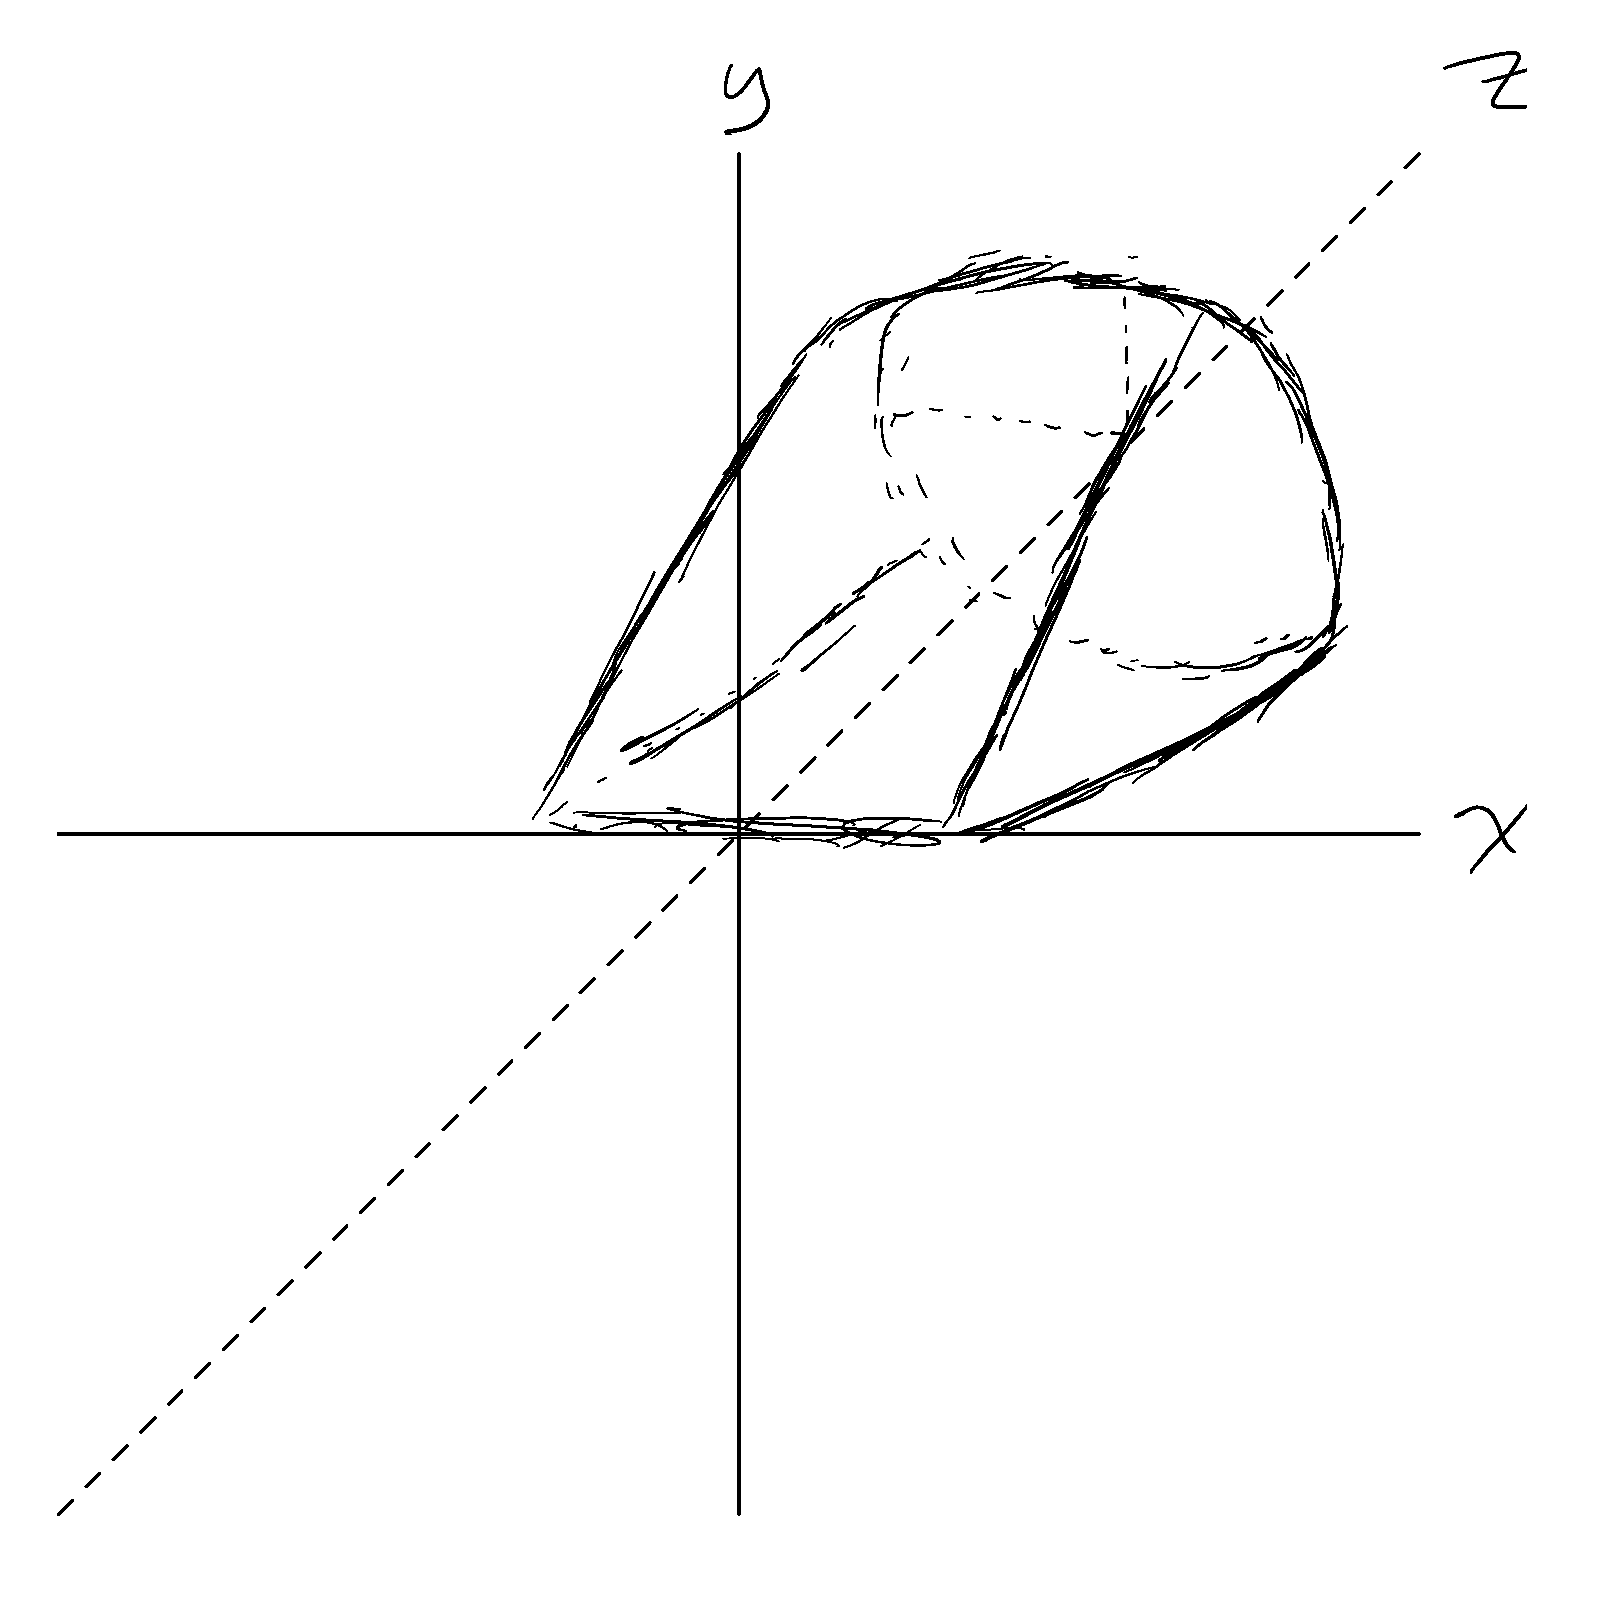
\includegraphics[scale=0.25]{q2bw.png}
	\end{figure}
\section{}
	The equation for a sphere is ${(x-a)}^2+{(y-b)}^2+{(z-c)}^2=r^2$ and describes a sphere of radius $r$
	centred at $(a,b,c)$.
	\begin{align*}
		|\vec{r}-\vec{r_o}|&=1\\
		\sqrt{{(x-x_o)}^2+{(y-y_o)}^2+{(z-z_o)}^2}&=1\\
		{(x-x_o)}^2+{(y-y_o)}^2+{(z-z_o)}^2&=1\\
	\end{align*}
	This fits the aforementioned equation for a sphere, and so the set of points $(x,y,z)$
	that satisfy $|\vec{r}-\vec{r_o}|=1$ describes a sphere of radius $1$ centred at $(x_o,y_o,z_o)$.
\section{}
	$AB$ is the diameter of a circle centred at $O$, so $A$'s $x$ component must be the additive inverse
	of $B$'s $x$ component and the same must be true of their $y$ components. Since $A$ sits on the curve of
	a circle, let it be defined as $A=(r\sin{t},r\cos{t})$ where $r$ is the radius of the circle and $t$ is
	some constant in the interval $[0,2\pi]$. By our definition, $B$ must be defined as $B=(-r\sin{t},-r\cos{t})$.
	$C$ is a point on the same circle, so let it be defined as $C=(r\sin{s},r\cos{s})$, where $s$ is some constant
	in the interval $[0,2\pi]$.
	\begin{align*}
		\vec{CA}=<r\sin{t}-r\sin{s},r\cos{t}-r\cos{s}>\\
		\vec{CB}=<-r\sin{t}-r\sin{s},-r\cos{t}-r\cos{s}>
	\end{align*}
	If $\vec{CA}\cdot{\vec{CB}}$ can be shown to be equal to $0$, then $\vec{CA}$ and $\vec{CB}$ are perpendicular.
	\begin{align*}
		\vec{CA}\cdot{\vec{CB}}&={(r\sin{t}-r\sin{s})}{(-r\sin{t}-r\sin{s})}+{(r\cos{t}-r\cos{s})}{(-r\cos{t}-r\cos{s})}\\
		&\begin{aligned}
			={(r\sin{t})}&{(-r\sin{t})}+{(r\sin{t})}{(-r\sin{s})}+{(-r\sin{s})}{(-r\sin{t})}+{(-r\sin{s})}^2+\\
		&{(r\cos{t})}{(-r\cos{t})}+{(r\cos{t})}{(-r\cos{s})}+{(-r\cos{s})}{(-r\cos{t})}+{(-r\cos{s})}^2
		\end{aligned}\\
		&=-r^2\sin^2{t}+r^2\sin^2{s}-r^2\cos^2{t}+r^2\cos^2{s}\\
		&=r^2{(\sin^2{s}+\cos^2{s})}-r^2{(\sin^2{t}+\cos^2{t})}\\
		&=r^2{(1)}-r^2{(1)}\\
		&=r^2-r^2\\
		&=0
	\end{align*}
\section{}
	\begin{align*}
		L_1&=(-2,0,-3)-(-4,-6,1)=(2,6,-4)\\
		L_2&=(5,3,14)-(10,18,4)=(-5,-15,10)\\
	\end{align*}
	The cross product of two vectors is a vector orthogonal to both. If the cross product of
	two vectors is $\vec{0}$, the two vectors are parallel, otherwise they are not parallel.
	\begin{align*}
		L_1\times{L_2}&=\langle60-60,-{(20-20)},-30-{(-30)}\rangle\\
		&=\langle0,0,0\rangle
	\end{align*}
	So $L_1$ and $L_2$ are parellel.
\section{}
	If the vectors normal to the two planes are orthogonal, then the two planes themselves are orthogonal.
	Vectors normal to the plane can be found by taking the coefficients of $x$, $y$, and $z$ in the plane's equation.
	\begin{align*}
		x+4y-3z=1\implies\langle1,4,-3\rangle\\
		-3x+6y+7z=0\implies\langle-3,6,7\rangle\\
	\end{align*}
	\begin{align*}
		\langle1,4,-3\rangle\cdot\langle-3,6,7\rangle&=-3+24-21\\
		&=0
	\end{align*}
	So the planes are orthogonal.
\section{}
	If each of the two lines' components share the same value for some $t$ in the interval, then
	the particles will collide. So if we set each set of components to be equal and solve for $t$,
	then any value of $t$ such that each set of components is equal will be a point at which the particles
	collide.\\
	The first set of components:
	\begin{align*}
		t^2=4t-3\\
		t^2-4t+3=0\\
		t=\frac{4\pm\sqrt{16-12}}{2}\\
		t=1,3
	\end{align*}
	The second set of components:
	\begin{align*}
		t^2=7t-12\\
		t^2-7t+12=0\\
		t=\frac{7\pm\sqrt{49-48}}{2}\\
		t=3,4
	\end{align*}
	The third set of components:
	\begin{align*}
		t^2=5t-6\\
		t^2-5t+6=0\\
		t=\frac{5\pm\sqrt{25-24}}{2}\\
		t=2,3
	\end{align*}
	So since each component intersects at $t=3$ (and since $3\ge0$), the particles will collide at when $t=3$.
\section{}
	\begin{align*}
		\frac{d}{dt}|\vec{r}(t)|&=\frac{d}{dt}\sqrt{\vec{r}(t)\cdot\vec{r}(t)}\\
		&=\frac{1}{2}{\bigg(\vec{r}(t)\cdot\vec{r}(t)\bigg)}^{-\frac{1}{2}}\cdot\frac{d}{dt}{\bigg(\vec{r}(t)\cdot\vec{r}(t)\bigg)}&\text{(Chain Rule)}\\
		&=\frac{1}{2}\cdot\frac{1}{{\bigg(\vec{r}(t)\cdot\vec{r}(t)\bigg)}^{\frac{1}{2}}}\cdot\frac{d}{dt}{\bigg(\vec{r}(t)\cdot\vec{r}(t)\bigg)}\\
		&=\frac{1}{2}\cdot\frac{1}{{\bigg(|\vec{r}(t)|^2\bigg)}^{\frac{1}{2}}}\cdot\frac{d}{dt}{\bigg(\vec{r}(t)\cdot\vec{r}(t)\bigg)}\\
		&=\frac{1}{2}\cdot\frac{1}{|\vec{r}(t)|}\cdot\frac{d}{dt}{\bigg(\vec{r}(t)\cdot\vec{r}(t)\bigg)}\\
		&=\frac{1}{2}\cdot\frac{1}{|\vec{r}(t)|}\cdot{\bigg(\vec{r'}(t)\cdot\vec{r}(t)+\vec{r}(t)\cdot\vec{r'}(t)\bigg)}&\text{(Product Rule)}\\
		&=\frac{1}{2}\cdot\frac{1}{|\vec{r}(t)|}\cdot2{\bigg(\vec{r'}(t)\cdot\vec{r}(t)\bigg)}\\
		&=\frac{2}{2}\cdot\frac{1}{|\vec{r}(t)|}\cdot{\bigg(\vec{r'}(t)\cdot\vec{r}(t)\bigg)}\\
		&=\frac{\vec{r'}(t)\cdot\vec{r}(t)}{|\vec{r}(t)|}
	\end{align*}
	Note that division by zero is undefined, and so $\vec{r}(t)$ cannot be $\vec{0}$.
\section{}
	Consider the vector function $\langle\sin{t},\cos{t},2\pi\rangle$.\\
	One full rotation of the circle (which has radius $1$) on the $xy$-axis formed by $\sin{t}$ and $\cos{t}$ takes $2\pi\cdot{t}$. In
	other words, each helix rises $2\pi\cdot{t}$ for every full rotation of the circle. The function can easily be modified to gain the
	properties that we want as follows:
	\begin{align*}
		\vec{r}(t)&=\bigg\langle10\sin{t},10\cos{t},\frac{34}{2\pi}\bigg\rangle\\
		&=\bigg\langle10\sin{t},10\cos{t},\frac{17}{\pi}\bigg\rangle
	\end{align*}
	Since each rotation takes $2\pi\cdot{t}$, $2.9\times10^8$ rotations will take $2\pi\cdot2.9\times10^8\cdot{t}$.\\
	The length of these helices can be found by calculating the arc length of one of them:
	\begin{align*}
		\int\displaylimits_{0}^{2.9\times10^8\cdot2\pi}|\vec{r}(t)|dt&=\int\displaylimits_{0}^{2.9\times10^8\cdot2\pi}\sqrt{{(10\cos{t})}^2+{(10\sin{t})}^2+{(\frac{17}{\pi})}^2}dt\\
		&=\int\displaylimits_{0}^{2.9\times10^8\cdot2\pi}\sqrt{10^2+{\bigg(\frac{17}{\pi}\bigg)}^2}dt\\
		&=\left. \sqrt{10^2+{\bigg(\frac{17}{\pi}\bigg)}^2}\cdot{t}\right\rvert_{0}^{2.9\times10^8\cdot2\pi}\\
		&=\sqrt{10^2+{\bigg(\frac{17}{\pi}\bigg)}^2}\cdot{2.9\times10^8\cdot2\pi}\\
		&=20717941308\\
		&\approx2.07\times10^{10}
	\end{align*}
	So the length of each helix is approximately $2.07\times10^{10}$\AA.\@

\end{document}
